\documentclass{book}

\usepackage[latin1]{inputenc} % para que TeX reconozca acentos, e�es y signos ��
                              % puestos directamente en el texto

\usepackage[T1]{fontenc} % para que los acentos y las e�es sean
\usepackage{lmodern}     % s�mbolos tomados directamente de los tipos
                         % de letras y no caracteres compuestos.

\usepackage[spanish,mexico]{babel} % para que palabras como "Chapter" salgan
                            % en espa�ol y se usen los patrones de
                            % divisi�n de palabras.

\usepackage{amsmath,amsfonts}

\usepackage[margin=3cm]{geometry}

\usepackage{macrosohm} % nuestros macros

\title{Olimpiada de Matem�ticas en Hidalgo\\ Problemas resueltos}
\author{Comit� ol�mpico de Matem�ticas en Hidalgo}

\begin{document}

\frontmatter

\maketitle

\tableofcontents


\chapter*{Introducci�n}
\label{cha:introduccion}

En este libro se incluyen los ex�mentes aplicados en las olimpiadas
estatales de matem�ticas del estado de Hidalgo, desde 2007 a la fecha.



%%% Local Variables: 
%%% mode: latex
%%% TeX-master: "libro"
%%% End: 

\mainmatter

\chapter{2007}
\label{cha:2007}

\begin{Problema}{1}
  Calcular el valor de
  \begin{equation}
    \label{eq:1}
    \sqrt{1+3+5+7+\cdots+2003+2005+2007},
  \end{equation}
  donde la suma dentro de la ra�z cuadrada es la suma de todos los
  n�meros impares del 1 al 2007.
\end{Problema}

\begin{Solucion}
  La suma $1+3+\cdots+(2n-1)$ de los primeros $n$ n�meros impares es
  igual a $n^{2}$. Si $2n-1=2007$ entonces $n=1004$, por lo que la
  suma~\ref{eq:1} vale $1004^{2}$.
\end{Solucion}

\begin{Problema}{2}
  Encuentre el volumen de un cono truncado de altura $2$, que tiene
  base inferior de radio $4$ y base superior de radio $3$ (ver la
  figura).
\end{Problema}

\begin{Solucion}
 La f\'ormula de volumen del cono es   
\end{Solucion}

\begin{Problema}{3}
  Considere un tri�ngulo de lados $a$, $b$ y $c$. Tome un punto $P$
  cualquiera en el interior del tri�ngulo y desde este punto trace
  segmentos perpendiculares a cada uno de sus lados. Suponga que $x$,
  $y$ y $z$ son las longitudes de estos segmentos perpendiculares a
  los lados $a$, $b$ y $c$, respectivamente. Demuestre que el �rea
  $A$ del tri�ngulo es igual a
  \begin{equation}
    \label{eq:2}
    A=\frac{1}{2}( ax+by+cz). 
  \end{equation}
\end{Problema}

\begin{Solucion}
  
\end{Solucion}

\begin{Problema}{4}
  Del siguiente diagrama calcule de cuantas maneras distintas se puede
  llegar del punto $A$ al punto $B$, respetando las direcciones de las
  flechas.
\[
\SelectTips{xy}{12}
\newdir{|>}{!/4.5pt/@{>}*:(1,-.2)@^{}*:(1,+.2)@_{}}
\entrymodifiers={-<5pt>}
\xymatrix{
 & & & & & &   &       &       &  \bullet   &\bullet\ar@{-|>}[l]_>*+{B}     \\ 
 & & & & & &   &       &       & \bullet\ar@{-|>}[u] &\bullet\ar@{-|>}[l]\ar@{-|>}[u]\\
 & & & & & &   &       &       &  \bullet\ar@{-|>}[u] &\bullet\ar@{-|>}[l]\ar@{-|>}[u]\\
 & & & & & &   &       &       & \bullet \ar@{-|>}[u] &\bullet\ar@{-|>}[l]\ar@{-|>}[u] \\
 & & & & & &   &       &       & \bullet\ar@{-|>}[u] &\bullet\ar@{-|>}[l]\ar@{-|>}[u] \\
 & & & & & &   &       &       & \bullet\ar@{-|>}[u]  &\bullet\ar@{-|>}[l]\ar@{-|>}[u]   \\
 & & & & & &   &       &       & \bullet\ar@{-|>}[u]  &\bullet\ar@{-|>}[l]\ar@{-|>}[u]   \\
 & & & & & &   &      &        & \bullet \ar@{-|>}[u] &\bullet\ar@{-|>}[l]\ar@{-|>}[u]   \\
 & & & & & &   &       &       & \bullet \ar@{-|>}[u] &\bullet\ar@{-|>}[l]\ar@{-|>}[u]   \\
 \bullet\ar@{-|>}[r]\ar@{-}[uuuuuuuuurrrrrrrrr]\ar@{->}[ur]&
 \bullet\ar@{-|>}[r]\ar@{-}[uuuuuuuurrrrrrrr]\ar@{->}[ur]&
 \bullet\ar@{-|>}[r]\ar@{-}[uuuuuuurrrrrrr]\ar@{->}[ur]&
 \bullet\ar@{-|>}[r]\ar@{-}[uuuuuurrrrrr]\ar@{->}[ur]&
 \bullet\ar@{-|>}[r]\ar@{-}[uuuuurrrrr]\ar@{->}[ur]&
 \bullet\ar@{-|>}[r]\ar@{-}[uuuurrrr]\ar@{->}[ur]&
 \bullet\ar@{-|>}[r]\ar@{-}[uuurrr]\ar@{->}[ur]&
 \bullet\ar@{-|>}[r]\ar@{-}[uurr]\ar@{->}[ur]&
 \bullet\ar@{-|>}[r]\ar@{-|>}[ur]&
 \bullet\ar@{-|>}[u]& 
 \bullet \ar@{-|>}[l]\ar@{-|>}[u] \\
\bullet\ar@{-|>}[r]_<*+{A}\ar@{-|>}[u] & \bullet\ar@{-|>}[r]\ar@{-|>}[u]& \bullet\ar@{-|>}[r]\ar@{-|>}[u]& \bullet\ar@{-|>}[r]\ar@{-|>}[u] & \bullet\ar@{-|>}[r]\ar@{-|>}[u]& \bullet \ar@{-|>}[r]\ar@{-|>}[u] & \bullet  \ar@{-|>}[r]\ar@{-|>}[u] &\bullet \ar@{-|>}[r]\ar@{-|>}[u]&\bullet\ar@{-|>}[u]\ar@{-|>}[r] &\bullet\ar@{-|>}[r]\ar@{-|>}[u] & \bullet  \ar@{-|>}[u] \\
 }
\]
\end{Problema}

\begin{Solucion}
  
\end{Solucion}

\begin{Problema}{5}
  Considere la ecuaci�n de segundo grado 
  \begin{equation}
    \label{eq:3}
    x^2-15ax+a^2=0.
  \end{equation}
  Encuentre todos los valores de $a$ de modo que las soluciones $x_1$
  y $x_2$ de esta ecuaci�n satisfacen
  \begin{equation}
    \label{eq:4}
    x_1^2+x_2^2=2007.
  \end{equation}
\end{Problema}

\begin{Solucion}
  Completando cuadrados en la ecuaci\'on \eqref{eq:3} tenemos que 
$$
x^2-14ax+\left(\frac {15} {2}a\right)^2=\frac{221} {4} a^2
$$
de donde se sigue que 
$$
\left(x-\frac {15} {2}a\right)^2=\frac{221} {4} a^2.
$$
Despejando la variable $x$, se tiene que las soluciones de la ecuaci\'on est\'an dadas por
$$
x_1=\frac a 2 (15+\sqrt{221})\qquad\qquad  x_2=\frac a 2 (15-\sqrt{221}).
$$
De esta forma, la ecuaci\'on \eqref{eq:4} toma la forma
$$
\frac {a^2} 4 \Bigl[\left(15+\sqrt{221}\right)+\left(15-\sqrt{221}\right)\Bigr]=2007.
$$
Despejando $a^2$ y haciendo las operaciones aritm\'eticas, se obtiene que $a^2=9$, de donde podemos concluir quedaron
los valores posibles de $a$ son $3$ y $-3$.
\end{Solucion}

\begin{Problema}{6}
  �De cu�ntas maneras se pueden sacar 10 canicas de una bolsa que
  contiene 7 canicas rojas, 8 azules y 7 verdes, si una vez que se
  sacaron no importa en que orden quedaron?
\end{Problema}

\begin{Solucion}
  
\end{Solucion}

%%% Local Variables: 
%%% mode: latex
%%% TeX-master: "libro"
%%% End: 

\chapter{2008}
\label{cha:2008}

\begin{Problema}{1}
  Jorge Luis cort� un cuadrado de papel que ten�a 20cm de per�metro y
  obtuvo dos rect�ngulos. Si el per�metro de uno de los rect�ngulos es
  16cm �cu�l es el per�metro del otro?
\end{Problema}

\begin{Solucion}
  
\end{Solucion}

\begin{Problema}{2}
  Un granjero descubre que si cuenta sus ovejas de dos en dos, o de
  tres en tres, o de cuatro en cuatro o de cinco en cinco, siempre le
  sobra una. Si el granjero tiene menos de cien ovejas y m�s de una,
  �cu�ntas ovejas tiene el granjero?
\end{Problema}

\begin{Solucion}
  
\end{Solucion}

\begin{Problema}{3}
  Denotemos por $f(n)$ la suma de los divisores positivos de un numero
  natural $n$. Por ejemplo, si~$n=6$ tenemos que los divisores de 6
  son 1,2,3 y 6, que sumados dan $f(6)=1+2+3+6=12$. Encuentra el valor
  de $f(n)$ m�s peque�o entre todas las $n$ mayores o iguales a 2008.
\end{Problema}

\begin{Solucion}
  
\end{Solucion}

\begin{Problema}{4}
  De una lista de~8 n�meros naturales consecutivos, se borra uno de
  los n�meros. La suma de los n�meros que quedaron despu�s de borrar
  es igual a 2008 �Cu�l es el n�mero borrado?
\end{Problema}

\begin{Solucion}
  
\end{Solucion}

\begin{Problema}{5}
  Considera el conjunto $A=\{1,2,3,\ldots,10\}$.  De cada subconjunto
  de 7 elementos de $A$ se toma el n�mero mayor �Cu�l es la suma de
  todos estos n�meros mayores?
\end{Problema}

\begin{Solucion}
  
\end{Solucion}

\begin{Problema}{6}
  Considera un cuadrado cuyo lado tiene longitud~$2$ y cuatro
  c�rculos del mismo radio con centros respectivos en los puntos
  medios del cuadrado, de tal modo que los c�rculos correspondientes a
  lados adyacentes son tangentes.  Encontrar el �rea de la regi�n
  dentro del cuadrado y fuera de los c�rculos. Es decir, en la figura
  siguiente, se pide hallar el �rea de la regi�n sombreada.

  \begin{center}
    \pgfmathsetmacro{\rad}{0.5*sqrt(2)}

    \begin{tikzpicture}[scale=1.2]
      \pgfmathparse{sqrt(2)*0.5}
      \filldraw[fill=gray,even odd rule]
      rectangle (2,2) (0,1)
      circle (\rad) (1,0)
      circle (\rad) (1,2)
      circle (\rad) (2,1)
      circle (\rad);
      \filldraw [fill=white]
      (0,1) circle (\rad)
      (1,0) circle (\rad)
      (1,2) circle (\rad)
      (2,1) circle (\rad);
      \draw rectangle (2,2);
    \end{tikzpicture}
  \end{center}
\end{Problema}


%%% Local Variables: 
%%% mode: latex
%%% TeX-master: "libro"
%%% End: 
\chapter{2009}
\label{cha:2009}

\begin{Problema}{1}
  Tenemos 120 esferas navide�as id�nticas metidas en cajitas del mismo
  tama�o.  Cada cajita contiene el mismo n�mero de esferas y el n�mero
  de esferas en cada cajita supera en 2 al n�mero de cajitas. �Cu�ntas
  cajitas hay y cu�ntas esferas hay dentro de cada cajita?
\end{Problema}

\begin{Solucion}
  
\end{Solucion}

\begin{Problema}{2}
  Suponga que $n\geq 1$ es un n�mero natural. Suponga que $n+1$ puede
  escribirse como la suma de los cuadrados de dos n�meros
  consecutivos, es decir, $n+1=m^2+(m+1)^2$ para alg�n n�mero natural
  $m$. Demuestre que $\sqrt{2n+1}$ es un n�mero entero impar.
\end{Problema}

\begin{Solucion}
  
\end{Solucion}

\begin{Problema}{3}
  En un tri�ngulo rect�ngulo con catetos de longitud $a$ y $b$ est�
  inscrito un cuadrado de tal manera que el cuadrado y el tri�ngulo
  comparten el �ngulo recto y un v�rtice del cuadrado est� sobre la
  hipotenusa. Hallar el per�metro del cuadrado.
\end{Problema}

\begin{Solucion}
  
\end{Solucion}

\begin{Problema}{4}
  �De cu�ntas maneras diferentes se pueden dar 100 pesos en cambio
  utilizando �nicamente monedas de 10 pesos, 5 pesos y 1 peso?
\end{Problema}

\begin{Solucion}
  
\end{Solucion}

\begin{Problema}{5}
  En una fiesta cada persona salud� a exactamente otras tres personas.
  \begin{itemize}
  \item Explique por qu� es imposible que a la fiesta hayan asistido
    exactamente~2009 personas.
  \item Si hubo en total~123 saludos, �cu�ntas personas asistieron a
    la fiesta?
  \end{itemize}
\end{Problema}

\begin{Solucion}
  La primera observaci\'on es que todo saludo es rec\'iproco, es
  decir, si Juan saluda a Pedro, tambi\'en Pedro saluda a
  Juan. Entonces ya que asistieron 2009 personas, cada una salud\'o
  exactamente a tres personas, pero podemos ver que cada saludo es
  contado dos veces, retomando el ejemplo anterior, es contado una vez
  cuando Juan saluda a Pedro y una segunda vez cuando Pedro saluda a
  Juan, debido a que son el mismo caso, tenemos que dividir el
  n\'umero de saludos entre dos, por lo que deber\'ia haber
  $\tfrac{2009\times 3}{2}=3013.5$ lo cual no es posible ya que el
  n\'umero de saludos tiene que ser un n\'umero entero.

  Ahora para el segundo inciso, realizaremos un razonamiento similar,
  si el total de saludos es 123, al multiplicar por dos \'este
  n\'umero deber\'ia ser igual al n\'umero de personas multiplicado
  por tres, retomando lo que se aplic\'o para resolver el inciso
  anterior, por lo tanto $123\times 2=246$ debe ser el triple de las
  personas que asistieron a la fiesta, por lo que hay
  $\tfrac{246}{3}=82$ personas, lo que se puede comprobar realizando
  el mismo proceso que en el inciso anterior para encontrar el
  n\'umero de saludos conociendo el n\'umero de personas.
\end{Solucion}

\begin{Problema}{6}
  En una granja hay un granero cuadrangular de 20 metros de
  lado. Una vaca est� atada a una de las paredes del granero, a 5
  metros de una esquina, con una soga de 10 metros de longitud.
  Calcule la superficie total sobre la cual la vaca puede pastar (la
  vaca s�lo puede pastar fuera del granero).
\end{Problema}

\begin{Solucion}
  
\end{Solucion}

%%% Local Variables: 
%%% mode: latex
%%% TeX-master: "libro"
%%% End: 
\chapter{2010}
\label{cha:2010}



%%% Local Variables: 
%%% mode: latex
%%% TeX-master: "libro"
%%% End: 
\chapter{2011}
\label{cha:2011}

\section{Primera parte}
\label{sec:primera-parte}

\begin{Problema}{1}
  
\end{Problema}

\begin{Solucion}
  
\end{Solucion}

\begin{Problema}{2}
  
\end{Problema}

\begin{Solucion}
  
\end{Solucion}

\begin{Problema}{3}
  
\end{Problema}

\begin{Solucion}
  
\end{Solucion}

\begin{Problema}{4}
  
\end{Problema}

\begin{Solucion}
  
\end{Solucion}

\begin{Problema}{5}
  
\end{Problema}

\begin{Solucion}
  
\end{Solucion}

\begin{Problema}{6}
  
\end{Problema}

\begin{Solucion}
  
\end{Solucion}

\begin{Problema}{7}
  
\end{Problema}

\begin{Solucion}
  
\end{Solucion}

\begin{Problema}{8}
  
\end{Problema}

\begin{Solucion}
  
\end{Solucion}

\begin{Problema}{9}
  
\end{Problema}

\begin{Solucion}
  
\end{Solucion}

\begin{Problema}{10}
  
\end{Problema}

\begin{Solucion}
  
\end{Solucion}

\section{Segunda parte}
\label{sec:segunda-parte}

\begin{Problema}{11}
  
\end{Problema}

\begin{Solucion}
  
\end{Solucion}

\begin{Problema}{12}
  
\end{Problema}

\begin{Solucion}
  
\end{Solucion}

\begin{Problema}{13}
  
\end{Problema}

\begin{Solucion}
  
\end{Solucion}



%%% Local Variables: 
%%% mode: latex
%%% TeX-master: "libro"
%%% End: 
\chapter{2012}
\label{cha:2012}

\section{Primera parte}
\label{sec:primera-parte2012}

\begin{Problema}{1}
  El precio de un pastel era de $200$ pesos, pero subi\'o un
  $25\%$. Sobre ese nuevo precio, se puso en oferta. Result\'o que con
  la oferta, el pastel volvi\'o a costar $200$ pesos. ?`De cu\'anto
  fue la oferta?

  \begin{inparaenum}
  \item $23\%$ \esp
  \item $25\%$ \esp
  \item $20\%$ \esp
  \item $35\%$ \esp
  \item De otro porcentaje
  \end{inparaenum}
\end{Problema}

\begin{Solucion}
  El pastel primero subi� $(0.25)(200)=\frac{200}{4}=50$ pesos, por lo
  que el nuevo precio era $200+50=250$ pesos. Queremos ahora saber qu�
  porcentaje de 250 es 50 pesos. Puesto que el $x\%$ de 250 es
  $250(\frac{x}{100})$, debemos resolver $250(\frac{x}{100})=50$, de
  donde se obtiene $x=20$. Es decir, la oferta fue de un $20\%$.
\end{Solucion}

\begin{Problema}{2}
  En un torneo de ping-pong hay ocho jugadores. Si cada uno de ellos
  juega una vez contra cada uno de los otros siete, ?`cu\'antos
  partidos se juegan en total?

  \begin{inparaenum}
  \item $8$ \esp
  \item $56$ \esp
  \item $28$ \esp
  \item $49$ \esp 
  \item Otro n\'umero
  \end{inparaenum}
\end{Problema}

\begin{Solucion}
  Como cada jugador juega contra otros siete, en principio ser�an
  $8\cdot 7=56$ partidos. Pero el partido del jugador A contra el
  jugador B es el mismo que el del jugador B contra el jugador A, por
  lo que en realidad la cantidad de partidos es $\frac{8\cdot
    7}{2}=28$. 
\end{Solucion}

\begin{Problema}{3}
  Considera la sucesi\'on de numeros $1, 3, 7, 13, 21, \cdots\,$ (los
  puntos suspensivos significan que es una lista infinita de
  n\'umeros, por lo que no la podemos escribir toda). El n\'umero que
  aparece en el lugar $n$ lo puedes calcular con la f\'ormula
  $n^2-n+1$ (por ejemplo, el n\'umero que aparece en el quinto lugar
  es $5^2-5+1=21$). ?`Qu\'e n\'umero le sigue al $91$ en la
  sucesi\'on?

  \begin{inparaenum}
  \item El $91$ no est\'a en la sucesi\'on \esp
  \item $98$ \esp
  \item $109$ \esp
  \item $111$ \esp 
  \item Otro n\'umero distinto de los anteriores 
\end{inparaenum}
\end{Problema}

\begin{Solucion}
  Las solucion a la ecuaci�n cuadr�tica $n^{2}-n+1=91$ son $n=10$,
  $n=-9$, por lo que 91 ocupa el �ndice 10 en la sucesi�n, y el
  siguiente n�mero corresponde al $n=11$, es decir $11^{2}-11+1=111$.
\end{Solucion}

\begin{Problema}{4}
  Tres tristes tigres tragaban trigo en treinta tristes trastos en un
  trigal.  El primer tigre trag\'o el doble de tristes trastos de
  trigo que el segundo tigre, mientras que el segundo tigre trag\'o el
  triple de tristes trastos de trigo que el tercer tigre.  ?`Cu\'antos
  tristes trastos de trigo trag\'o el tercer tigre?

  \begin{inparaenum}
  \item $15$ \esp
  \item $10$ \esp
  \item $5$ \esp
  \item $20$ \esp
  \item Otro n\'umero de trastos
  \end{inparaenum}
\end{Problema}

\begin{Solucion}
  Si el tercer tigre trag� $x$ trastos, el segundo trag� $3x$ y el
  primero trag� $2(3x)=6x$. Es decir, en total se tragaron
  $6x+3x+x=10x=30$ trastos, por lo que $x=3$.
\end{Solucion}

\begin{Problema}{5}
  Considera un rect\'agulo cuyas longitudes de sus lados son n\'umeros enteros. Si 
  el \'area del rect\'angulo es 21, ?`cu\'ales son los posibles valores de sus lados?

  \begin{inparaenum}
  \item $20$ y $44$ \quad\qquad
  \item $15$ y $30$ \quad\qquad
  \item $17$ y $44$ \quad\qquad
  \item $10$ y $22$ \quad\qquad
  \item Otro par de valores
  \end{inparaenum}
\end{Problema}

\begin{Solucion}
  Los �nicos posibles valores para las longitudes de los lados son:
  21,1 o 3,7.
\end{Solucion}

\begin{Problema}{6}
  En un c\'irculo se encuentra inscrito un tri\'angulo equil\'atero, como en la figura. 
  Si el \'area del tri\'angulo es uno, ?`cu\'al es el valor del \'area de la regi\'on 
  sombreada?

  \begin{center}
    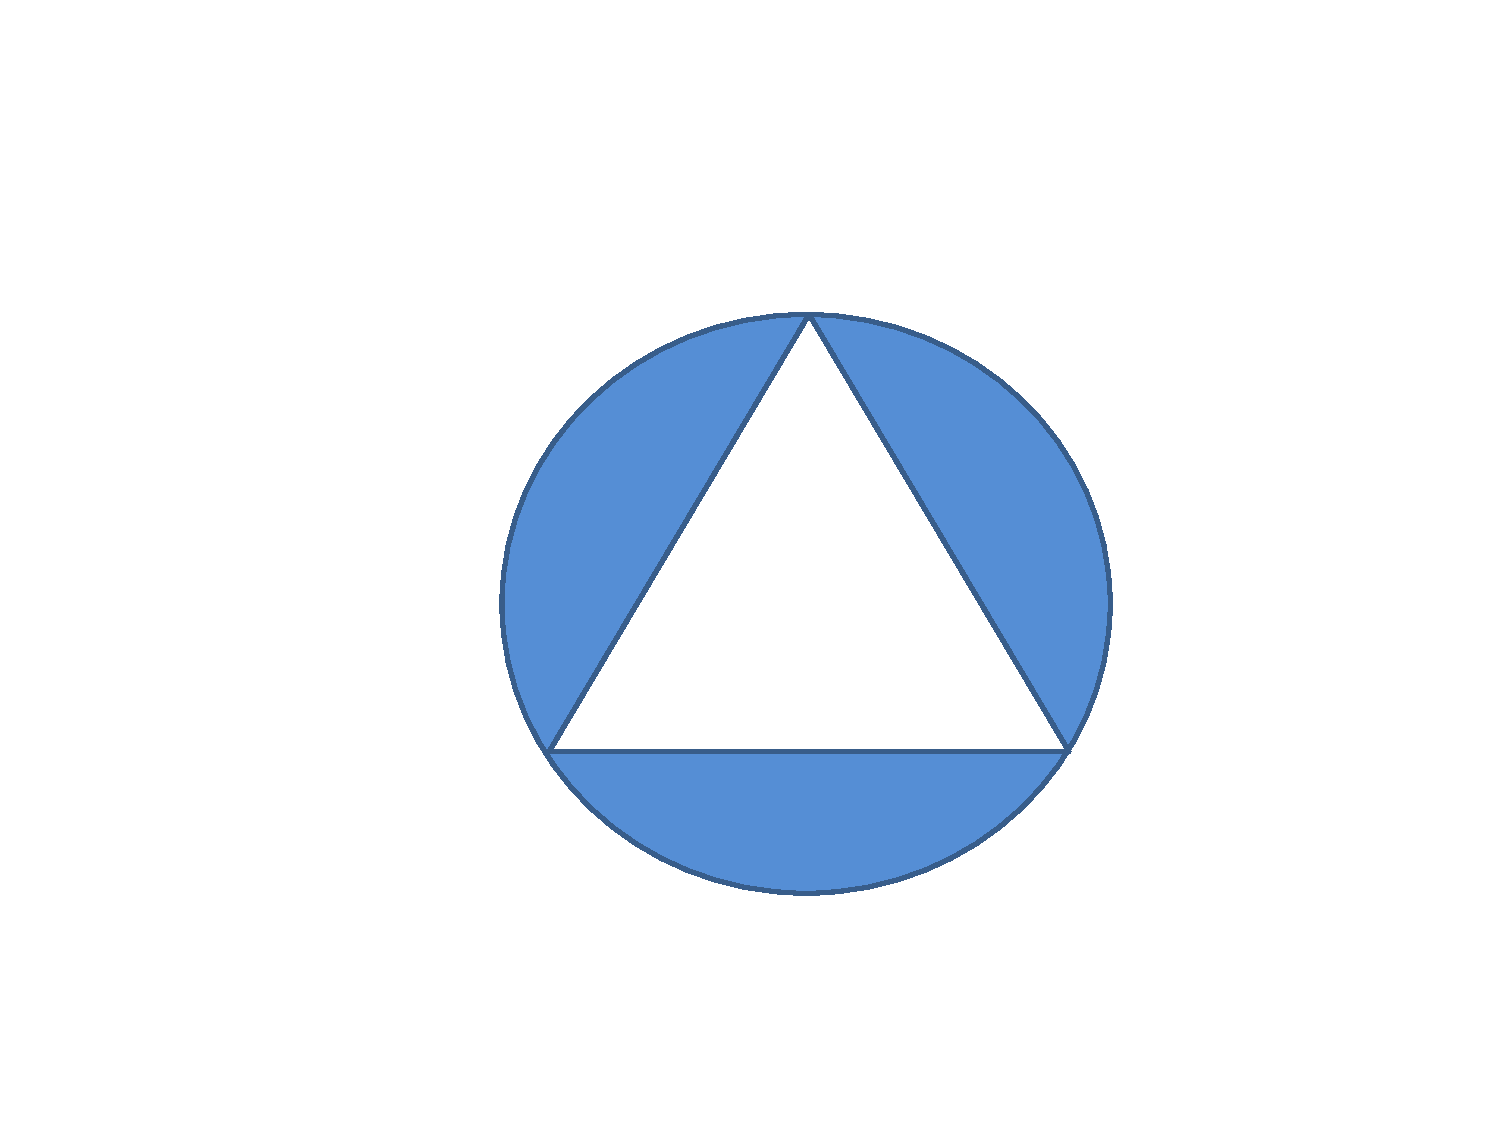
\includegraphics[scale=0.20]{critri.pdf}
  \end{center}

  \begin{inparaenum}
  \item $\dfrac{4\pi}{3\sqrt{3}}-1$, \quad\qquad
  \item $\dfrac{4\pi}{\sqrt{3\sqrt{3}}}-1$ \quad\qquad
  \item $\dfrac{4\pi}{9}-1$ \quad\qquad
  \item $\dfrac{4\pi}{3}-1$ \quad\qquad 
  \item Otro valor
  \end{inparaenum}
\end{Problema}

\begin{Solucion}
  Sea $r$ el radio del c�rculo. Queremos entonces expresar el �rea del
  tri�ngulo en funci�n de $r$, y para eso necesitamos a su vez
  expresar la base y la altura en funci�n de $r$.

  Partiendo del centro del c�rculo y trazando una perpedicular a un
  lado, formamos un peque�o tri�ngulo rect�ngulo que tiene un radio
  $r$ como hipotenusa. Dado que el tri�ngulo original es equil�tero,
  el segmento perpendicular trazado mide $\frac{r}{2}$, y por lo tanto
  el otro cateto mide $\frac{r\sqrt{3}}{2}$. Dado que este �ltimo
  cateto mide la mitad del lado del tri�ngulo original, tenemos que el
  tri�ngulo original tiene lado $r\sqrt{3}$ y altura $\frac{3r}{2}$,
  de donde se obtiene:
  \begin{equation}
    \label{eq:5}
    r^{2}=\frac{4}{3\sqrt{3}}.
  \end{equation}

  Por lo tanto, el �rea del c�rculo es $\pi\frac{4}{3\sqrt{3}}$, y el
  �rea sombreada es $\frac{4\pi}{3\sqrt{3}}-1$.
\end{Solucion}

\begin{Problema}{7}
  El ayuntamiento de Mineral de la Reforma te ha encargado pintar las
  cuatro caras exteriores de un monumento piramidal como el que se
  muestra en la figura. La pir\'amide es lisa, tiene una base cuadrada
  de 16 metros de lado y una altura de 6 metros. Una cubeta de pintura
  cuesta 900 pesos y con ella puedes pintar 40 metros
  cuadrados. ?`Cu\'anto cuesta toda la pintura que necesitas?

  \begin{center}
    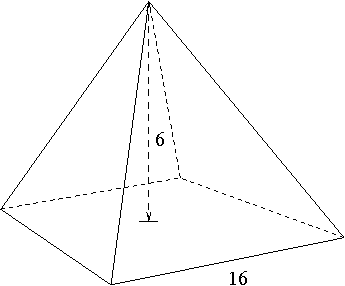
\includegraphics[scale=.44]{OHMpyramid.png}
  \end{center}

  \begin{inparaenum}
  \item $\$7,200$ \quad\qquad
  \item $\$12,960$ \quad\qquad
  \item $\$4,320$ \quad\qquad
  \item $\$10,800$ \quad\qquad
  \item Otra cantidad
  \end{inparaenum}
\end{Problema}

\begin{Solucion}
  
\end{Solucion}

\begin{Problema}{8}
  ?`Cu\'al es el valor m\'as grande que puede tomar la cantidad 
  $\displaystyle{(m+n)/n}$, si sabes que $m$ y $n$ son n\'umeros enteros positivos 
  tales que $n>99$ y $m<101$?

  \begin{inparaenum}
  \item 2 \esp
  \item 7 \esp
  \item 38 \esp
  \item 5 \esp
  \item Ninguno de los valores anteriores
  \end{inparaenum}
\end{Problema}

\begin{Solucion}
  
\end{Solucion}

\begin{Problema}{9}
  En una tina con agua como la de la figura, flota una pelota de $60$
  cent\'imetros de di\'ametro. Si el di\'ametro de la tina es de $180$
  cent\'imetros y exactamente un cuarto del volumen de la pelota se
  encuentra sumergida en la tina, ?`cu\'antos cent\'imetros bajar\'a
  el nivel del agua en el recipiente cuando se saque la pelota? El
  volumen total de la pelota es de $36,000\pi$ cm$^3$.

  \begin{center}
    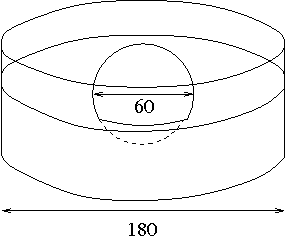
\includegraphics[scale=.58]{OHMballinpool.png}
  \end{center}

  \begin{inparaenum}
  \item $1$ cm\esp
  \item $\dfrac{\pi}{3}$ cm \esp
  \item $\dfrac{10}{9} $ cm\esp
  \item $\dfrac{\pi}{2}$\esp
  \item Otra cantidad
  \end{inparaenum}  
\end{Problema}

\begin{Solucion}
  
\end{Solucion}

\begin{Problema}{10}
  Chaco planea robar un banco y le promete darle al Roto un tercio del
  bot\'in si le ayuda. El Roto acepta, pero como no sabe manejar, le
  pide ayuda al Pepis a cambio de darle un tercio de lo que ganar\'a
  por el robo. El Pepis acepta, pero su auto est\'a en el taller,
  as\'i que le dice al Chueco que si le deja usar su auto, le dar\'a
  un tercio de lo que \'el gane. El Chueco acepta, pero como no oye
  bien, le dice al Pollo que si le ayuda le dar\'a un tercio de lo que
  gane. El Pollo acepta. Tres d\'ias despu\'es del robo atrapan al
  Chueco con su parte del bot\'in, que es de 40,000 pesos.  ?`Cu\'anto
  dinero se llevaron entre todos?

  \begin{inparaenum}
  \item \$810,000 \quad\quad
  \item \$3,240,000 \quad\quad
  \item \$1,620,000 \quad\quad
  \item \$1,000,000 \quad\quad 
  \item Otra cantidad
  \end{inparaenum}
\end{Problema}

\begin{Solucion}
  
\end{Solucion}

\section{Segunda parte}
\label{sec:segunda-parte2012}

\begin{Problema}{11}
  Paco y Luis se tienen que formar en una fila con sus compa\~neros
  Carlos, Miguel, Daniel y Joel. ?`De cu\'antas formas distintas se
  pueden acomodar de manera que entre Luis y Paco se encuentren
  formados exactamente dos de sus compa\~neros?
\end{Problema}

\begin{Solucion}
  
\end{Solucion}

\begin{Problema}{12}
  Si $c$ es la longitud de la hipotenusa de un tri\'angulo
  rect\'angulo cuyos otros dos lados tienen longitudes $a$ y $b$,
  muestra que $a+b\leq\sqrt{2}c$.
\end{Problema}

\begin{Solucion}
  
\end{Solucion}

\begin{Problema}{13}
  Considera un c\'irculo con centro $O$, como se muestra en la figura.
  $DEB$ es una cuerda del c\'irculo tal que $DE=3$ y $EB=5$. Si $AC$
  es un di\'ametro del c\'irculo que pasa por el punto $E$ y $EC=1$,
  ?`cu\'anto debe medir el radio del c\'irculo?

  \begin{center}
    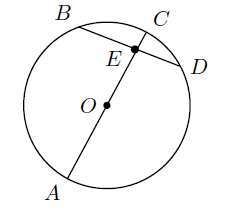
\includegraphics[scale=0.85]{problema2.png}
  \end{center}
\end{Problema}

\begin{Solucion}
  
\end{Solucion}


%%% Local Variables: 
%%% mode: latex
%%% TeX-master: "libro"
%%% End: 
\chapter{2013}
\label{cha:2013}

\section{Primera parte}
\label{sec:primera-parte2013}

\begin{Problema}{1}
  ?`Cu\'al es el \'ultimo d\'igito del n\'umero $(2013)^{2014}$?

  \begin{inparaenum}
  \item 1 \espl
  \item 3 \espl
  \item 5 \espl
  \item 7 \espl
  \item 9
  \end{inparaenum}
\end{Problema}

\begin{Problema}{2}
  Un c\'irculo de radio $1$ est\'a inscrito en un tri\'angulo
  equil\'atero. El tri\'angulo, a su vez, est\'a ins\-cri\-to en otro
  c\'irculo.  Calcula el \'area entre los dos c\'irculos (el \'area
  sombreada en la figura).

  \begin{inparaenum}
  \item $\pi$ \espm
  \item $\sqrt{3} \pi$ \espm
  \item $2 \pi$ \espm
  \item $3 \pi$ \espm
  \item \nota.
  \end{inparaenum}

%  \begin{figure}[!htbp]
  % \begin{center}
  %   \begin{pspicture}(-1.6,-1.6)(1.6,1.6)\psset{unit=0.8cm}
  %     \pscircle[fillstyle=solid,fillcolor=lightgray]{2}\pscircle[fillstyle=solid,fillcolor=white]{1}
  %     \pspolygon(0,2)(1.732,-1)(-1.732,-1)(0,2)\psline[linestyle=dashed]{*->}(1,0)\uput[d](0.5,0){$1$}
  %   \end{pspicture}
  %   \end{center}
%  \end{figure}
\end{Problema}

\begin{Problema}{3}
Se tiene una cuarta parte de un c\'irculo de radio $2$. Inscrito
  en \'el, como se ve en la figura, est\'a otro c\'irculo. ?`Cual es el per\'imetro del c\'irculo peque\~no?

\begin{inparaenum}
\item $\pi$ \espc
\item $2 \pi$ \espc
\item $\frac{2}{1+\sqrt{2}} \pi$ \espm
\item $\frac{4}{1+\sqrt{2}} \pi$ \espm
\item \nota.
\end{inparaenum}

% \begin{figure}[!htbp]
% \centering\begin{pspicture}(0,0)(1.6,1.6)\psset{unit=0.8cm}
%   \pswedge[fillstyle=solid,fillcolor=lightgray]{2}{0}{90}\pscircle[fillstyle=solid,fillcolor=white](0.828427,0.828427){0.828427}
%   \psline(-0.4,2)(-0.2,2)\psline(-0.4,0)(-0.2,0)\psline[linestyle=dashed]{<->}(-0.3,2)(-0.3,0)\uput[l](-0.3,1){$2$}
% \end{pspicture}
% \end{figure}
\end{Problema}

\begin{Problema}{4}
  En Actopan hay una cerca con forma de tri\'angulo equil\'atero
  que mide $6$ metros por lado y que protege un campo de
  alfalfa. Afuera del tri\'angulo hay un borrego atado 
 con una cuerda de $3$ metros de longitud a un poste de la cerca. Si el poste
  est\'a a $2$ metros de una de las esquinas, ?`cu\'al es el tama\~no
  del \'area total en la que el borrego puede pastar?


\begin{inparaenum}
\item $5\pi$ \espm
\item $\frac{5}{3}\pi$ \espm
\item $\frac{29}{5} \pi$ \espm
\item $\frac{29}{6} \pi$ \espm
\item \nota.
\end{inparaenum}
\end{Problema}

\begin{Problema}{5}
  Calcula el valor de
$$
\frac{123456789}{(-123456789)^2+(-123456788)(123456790)}
$$

\begin{inparaenum}
\item $123456788$ \espsc
\item $123456789$ \espsc
\item $123456790$ \espsc
\item $\frac{1}{2\times123456789}$ \espsc
\item \nota.
\end{inparaenum}
\end{Problema}

\begin{Problema}{6}
  Dadas $6$ rectas distintas en el plano, ?`cu\'al es el n\'umero
  m\'aximo de puntos en los que pueden intersectarse?

\begin{inparaenum}
\item $6$ \espm
\item $10$ \espm
\item $15$ \espm
\item $16$ \espm
\item \nota.
\end{inparaenum}
\end{Problema}

\begin{Problema}{7}
Se colocan $7$ c\'irculos de radio $1$ de manera que los centros
  est\'en en linea recta y sean tangentes, como se muestra en la
  figura. Calcula el \'area de la regi\'on sombreada.


\begin{inparaenum}
\item $24+\pi$ \espc
\item $24-6\pi$ \espc
\item $24-7\pi$ \espc
\item $28 -7\pi$ \espc
\item \nota.
\end{inparaenum}

% \begin{figure}[!htbp]
% \centering\begin{pspicture}(-6,-0.8)(6,0.8)\psset{unit=0.8cm}
%   \psframe[fillstyle=solid,fillcolor=lightgray](-6,-1)(6,1)
%   \pscircle[fillstyle=solid,fillcolor=white](0,0){1}\pscircle[fillstyle=solid,fillcolor=white](2,0){1}
%   \pscircle[fillstyle=solid,fillcolor=white](4,0){1}\pscircle[fillstyle=solid,fillcolor=white](6,0){1}
%   \pscircle[fillstyle=solid,fillcolor=white](-2,0){1}\pscircle[fillstyle=solid,fillcolor=white](-4,0){1}
%   \pscircle[fillstyle=solid,fillcolor=white](-6,0){1}\psline(-7.5,0)(7.5,0)\psline[linestyle=dashed]{*->}(0,0)(0,1)\uput[l](0,0.5){$1$}
%   \psline[linestyle=dashed]{*->}(2,0)(2,1)\uput[l](2,0.5){$1$}\psline[linestyle=dashed]{*->}(4,0)(4,1)\uput[l](4,0.5){$1$}
%   \psline[linestyle=dashed]{*->}(6,0)(6,1)\uput[l](6,0.5){$1$}\psline[linestyle=dashed]{*->}(-2,0)(-2,1)\uput[l](-2,0.5){$1$}
%   \psline[linestyle=dashed]{*->}(-4,0)(-4,1)\uput[l](-4,0.5){$1$}\psline[linestyle=dashed]{*->}(-6,0)(-6,1)\uput[l](-6,0.5){$1$}
% \end{pspicture}
% \end{figure}
  
\end{Problema}

\begin{Problema}{8}
  Considera un n\'umero de tres d\'igitos $abc$ y un n\'umero de
  dos d\'igitos $aa$. Si multiplicas estos dos n\'umeros se obtiene el $2013$. ?`Cu\'al
  es el valor de $a \times b \times c$?

\begin{inparaenum}
\item $30$ \espm
\item $183$ \espm
\item $671$ \espm
\item $2013$ \espm
\item \nota.
\end{inparaenum}
\end{Problema}

\begin{Problema}{9}
  En casa hay tres relojes. El 9 de febrero de 2013 a las 10:00am
  todos ellos indicaban la hora correctamente, pero solo marchaba bien
  el primer reloj. El segundo se atrasaba un minuto al d\'ia y el
  tercero se adelantaba un minuto al d\'ia. Si los relojes contin\'uan
  marchando as\'i, ?`al cabo de cu\'anto tiempo volver\'an los tres a
  marcar exactamente las 10:00am?

\begin{inparaenum}
\item $240$ d\'ias \espsc
\item $720$ d\'ias \espsc
\item $1440$ d\'ias \espsc
\item nunca lo har\'an \espsc
\item \nota.
\end{inparaenum}
\end{Problema}


\begin{Problema}{10}
La base de un rect\'angulo es el doble de su altura. Si la base
  se disminuye en $6$ unidades y la altura se aumenta en $4$ el \'area
  del rect\'angulo no cambia. ?`Cu\'al es el \'area del rect\'angulo?

\begin{inparaenum}
\item $1$ \espm
\item $24$ \espm
\item $144$ \espm
\item $288$ \espm
\item \nota.
\end{inparaenum}
\end{Problema}

\section{Segunda parte}
\label{sec:segunda-parte2013}

\begin{Problema}{11}
Decimos que tres enteros positivos $a$, $b$ y $c$ est\'an en
  progresi\'on aritm\'etica si $a < b < c$ y $b-a=c-b$. Supongamos que
  $a$, $b$ y $c$ son enteros positivos en progresi\'on
  aritm\'etica. Demuestra que
$$
\frac{1}{\sqrt{b}+\sqrt{c}}, \quad \frac{1}{\sqrt{c}+\sqrt{a}}, \quad \frac{1}{\sqrt{a}+\sqrt{b}}
$$
est\'an en progresi\'on aritm\'etica.
\end{Problema}

\begin{Problema}{12}
  Calcula el valor de
$$
(2+1)(2^2+1)(2^4+1)(2^8+1)(2^{16}+1)(2^{32}+1)(2^{64}+1)(2^{128}+1)(2^{256}+1)(2^{512}+1)(2^{1024}+1) + 1.
$$
\end{Problema}

\begin{Problema}{13}
En una cuarto de tama\~no rectangular se acomodan $m \times n$ sillas de
  manera rectangular de tal modo que se forman $m>1$ filas y $n>1$
  columnas de sillas. Entran los estudiantes al examen y cada uno se
  sienta en una silla, sin que queden sillas vac\'ias. Despu\'es, cada
  estudiante saluda de mano a los que est\'an junto a \'el (al que
  est\'a a su derecha, a su izquierda, adelante y atr\'as). Si en total
  se hicieron $275$ saludos, ?`cu\'antas sillas hay en el sal\'on?
\end{Problema}

%%% Local Variables: 
%%% mode: latex
%%% TeX-master: "libro"
%%% End: 

\chapter{2014}
\label{cha:2014}

\section{Primera parte}
\label{sec:primera-parte2014}

\begin{Problema}{1}
  �Cu�l es el valor de la suma de todos los enteros entre 50 y 350
  que terminan en 1?

  \respuestas{5880}{5850}{5208}{4877}{\nota}
\end{Problema}

\begin{Solucion}
\end{Solucion}

\begin{Problema}{2}
  \begin{minipage}[t]{0.6\linewidth}
    �De cu�ntas formas se puede llenar la siguiente cuadr�cula con 1 o
    $-1$, de forma que la suma de los n�meros en cada rengl�n y cada
    columna sea igual a 0?
  \end{minipage}
  \hspace*{\fill}
  \begin{minipage}[t]{0.35\linewidth}
    \vspace{-3mm}
    \centering
    \begin{tikzpicture}[scale=0.7]
      \draw[thick] (0,0) grid (8,2);
    \end{tikzpicture}
  \end{minipage}

  \respuestas{16}{32}{60}{70}{\nota}
\end{Problema}

\begin{Solucion}
\end{Solucion}

\begin{Problema}{3}
  \begin{minipage}[t]{0.6\linewidth}
    En la figura, el lado del cuadrado $ABCD$ mide 12cm. Adem�s, la
    longitud de $AP$ es 4cm, la de $DQ$ es 3cm y el $\angle RQC$ es
    recto. �Cu�nto mide el segmento $RB$?
  \end{minipage}
  \hspace*{\fill}
  \begin{minipage}[t]{0.35\linewidth}
    \vspace{-5mm}
    \centering
    \newcommand{\unidad}{3.343}
    \pgfmathsetmacro{\tercio}{\unidad*(1/3)}
    \pgfmathsetmacro{\cuarto}{\unidad*(1/4)}
    \begin{tikzpicture}
      \tkzDefPoint(0,0){D}
      \tkzDefPoint(0,\unidad){A}
      \tkzDefPoint(\unidad,\unidad){B}
      \tkzDefPoint(\unidad,0){C} 
      \tkzDefPoint(\tercio,\unidad){P} 
      \tkzDefPoint(\cuarto,0){Q} 
      \tkzDrawSegment(A,B)
      \tkzDrawSegment(B,C)
      \tkzDrawSegment(C,D)
      \tkzDrawSegment(A,D)
      \tkzDrawSegment(P,D)
      \tkzDefPointWith[orthogonal,K=1](Q,C) \tkzGetPoint{H}
      \tkzInterLL(Q,H)(D,P) \tkzGetPoint{R}
      \tkzDrawSegment(Q,R)
      \tkzLabelPoints[above left](R)
      \tkzLabelPoints[above](A,B,P)
      \tkzLabelPoints[below](D,C,Q)
      \tkzDrawPoints(A,B,C,D,P,Q,R) 
    \end{tikzpicture}
  \end{minipage}

  \respuestas{10}{11}{$3\sqrt{10}$}{$3\sqrt{11}$}{\nota}
\end{Problema}

\begin{Solucion}
  
\end{Solucion}

\begin{Problema}{4}
  Se tiene una bolsa con 44 bolas verdes, 53 blancas y 27 rojas. �Cu�l
  es el menor n�mero de bolas que hay que sacar, para garantizar que
  haya al menos cuatro bolas de cada color?

  \respuestas{12}{13}{101}{111}{\nota}  
\end{Problema}

\begin{Solucion}
  
\end{Solucion}

\begin{Problema}{5}
  La leche con chocolate Cuak contiene una parte de chocolate por
  cada nueve partes de leche. El chocolate l�quido con leche Mayoral
  contiente cuatro partes de chocolate por cada parte de leche. Se
  revuelve una porci�n de Cuak con otra porci�n de Mayoral para formar
  una mezcla de un litro. Si la mezcla que se obtiene contiene la
  misma cantidad de leche que de chocolate, �cu�nto de Cuak hay en la
  mezcla?

  \respuestas{$\frac{1}{4}$ de litro}{$\frac{15}{19}$ de  litro}%
  {$\frac{4}{7}$ de litro}{$\frac{3}{7}$ de litro}{\nota}
\end{Problema}

\begin{Solucion}
  
\end{Solucion}

\begin{Problema}{6}
  El valor de la suma (donde los puntos suspensivos representan
  todos los sumandos intermedios)
  $$
  1+2+3-4+5+6+7-8+\cdots+1997+1998+1999-2000
  $$
  es igual a:

  \respuestas{$1500000$}{$999000$}{$501100$}{$998900$}{\nota}
\end{Problema}

\begin{Solucion}
  
\end{Solucion}

\begin{Problema}{7}
  Dos trabajadores, Pepe y Paco, descargaron 2014 cajas de dulces
  de un cami�n. Pepe acarre� las cajas de seis en seis, mientras que
  Paco las acarre� de siete en siete. Si los dos trabajadores
  comenzaron a descargar al mismo tiempo, y Pepe dio dos vueltas por
  cada una que dio Paco, �cu�ntas vueltas dio Pepe?

  \respuestas{100}{106}{155}{212}{\nota}  
\end{Problema}

\begin{Solucion}
  
\end{Solucion}

\begin{Problema}{8}
  \begin{minipage}[t]{0.6\linewidth}
    En la siguiente figura se muestra un cuadrado inscrito dentro de
    un tri�ngulo equil�tero. Si el lado del tri�ngulo mide 2, �cu�nto
    mide el lado del cuadrado?
  \end{minipage}
  \hspace*{\fill}
  \begin{minipage}[t]{0.35\linewidth}
    \vspace{-5mm}
    \centering
    \newcommand{\unidad}{3.223}
    \pgfmathsetmacro{\cuad}{\unidad*(1/(sqrt(3)+2))}
    \begin{tikzpicture}
      \tkzDefPoint(0,0){A}
      \tkzDefPoint(\unidad,0){B}
      \tkzDefPoint(60:\unidad){C}
      \tkzDefPoint(\cuad,0){D}
      \tkzDefPointWith[orthogonal](D,B) \tkzGetPoint{E}
      \tkzInterLL(D,E)(A,C) \tkzGetPoint{F}
      \tkzDefPointWith[orthogonal](F,D) \tkzGetPoint{G}
      \tkzInterLL(B,C)(F,G) \tkzGetPoint{H}
      \tkzDefPointWith[orthogonal](H,F) \tkzGetPoint{I}
      \tkzInterLL(H,I)(A,B) \tkzGetPoint{J}
      \tkzDrawSegment(A,B)
      \tkzDrawSegment(B,C)
      \tkzDrawSegment(C,A)
      \tkzDrawSegment(D,F)
      \tkzDrawSegment(F,H)
      \tkzDrawSegment(H,J)
    \end{tikzpicture}        
  \end{minipage}

  \respuestas{$\frac{2\sqrt{3}}{\sqrt{3}+2}$}{$\frac{\sqrt{3}}{\sqrt{3}+4}$}{$\frac{\sqrt{2}}{2}$}{1}{\nota}  
\end{Problema}

\begin{Solucion}
  
\end{Solucion}

\begin{Problema}{9}
  \begin{minipage}[t]{0.6\linewidth}
    El rect�ngulo de la figura est� dividido en 8 regiones. Las �reas
    de tres regiones han sido marcadas. Encuentra el �rea de la regi�n
    marcada con ``?''.
  \end{minipage}
  \hspace*{\fill}
  \begin{minipage}[t]{0.35\linewidth}
    \vspace{-5mm}
    \centering
    \newcommand{\alto}{3}
    \pgfmathsetmacro{\ancho}{1.421*\alto}
    \pgfmathsetmacro{\derecha}{\alto*0.5478}
    \pgfmathsetmacro{\abajo}{\ancho*0.4314}
    \begin{tikzpicture}
      \tkzDefPoint(0,0){A}
      \tkzDefPoint(\ancho,0){B}
      \tkzDefPoint(\ancho,\alto){C}
      \tkzDefPoint(0,\alto){D} 
      \tkzDefPoint(\ancho,\derecha){N} 
      \tkzDefPoint(\abajo,0){M} 
      \tkzDefPoint(0.5*\ancho,0.5*\alto){X} 

      \tkzInterLL(D,M)(A,N) \tkzGetPoint{a}
      \tkzInterLL(C,M)(D,N) \tkzGetPoint{b}

      \tkzCentroid(A,M,a)\tkzGetPoint{x}\tkzLabelPoint[right](x){3}
      \tkzCentroid(B,M,N)\tkzGetPoint{y}\tkzLabelPoint[above left](y){20}
      \tkzInCenter(b,C,N)\tkzGetPoint{z}\tkzLabelPoint[above](z){2}
      \tkzLabelPoint[above left](X){?}

      \tkzDrawSegment(A,B)
      \tkzDrawSegment(A,D)
      \tkzDrawSegment(C,D)
      \tkzDrawSegment(B,C)
      \tkzDrawSegment(A,N)
      \tkzDrawSegment(D,N)
      \tkzDrawSegment(D,M)
      \tkzDrawSegment(C,M)
    \end{tikzpicture}
  \end{minipage}

  \respuestas{$12.5$}{$20$}{$25$}{\nota}{Falta informaci�n}
\end{Problema}

\begin{Solucion}
  
\end{Solucion}

\begin{Problema}{10}
  \begin{minipage}[t]{0.6\linewidth}
    En el tri�ngulo $ABC$, los lados $AC$, $AB$, $BC$, miden $x-1$,
    $x$, $x+1$ respectivamente. El punto $H$ es el pie de la altura en
    el lado $AB$. Si los segmentos $AH$, $HB$, miden $a$, $b$
    respectivamente, encuentra el valor de $b-a$.
  \end{minipage}
  \hspace*{\fill}
  \begin{minipage}[t]{0.35\linewidth}
    \vspace{-5mm}
    \centering
    \newcommand{\equis}{10}
    \pgfmathsetmacro{\coseno}{0.5*(\equis-4)/(\equis-1)}
    \pgfmathsetmacro{\angulo}{acos(\coseno)}
    \pgfmathsetmacro{\lado}{\equis-1}
    \usetkzobj{all}
    \begin{tikzpicture}[scale=0.4]
      \tkzDefPoint(0,0){A}
      \tkzDefPoint(\equis,0){B}
      \tkzDefPoint(\angulo:\lado){C}
      \tkzDefPointBy[projection=onto B--A](C) \tkzGetPoint{H}
      \tkzDrawSegment(A,B)
      \tkzDrawSegment(B,C)
      \tkzDrawSegment(C,A)
      \tkzDrawSegment(C,H)
      \tkzLabelPoints[below](A,B,H)
      \tkzLabelPoints[above](C)
      \tkzMarkRightAngle(B,H,C)
      \tkzDrawPoints(A,B,C,H) 
    \end{tikzpicture}
  \end{minipage}

  \respuestas{3}{4}{$2x$}{\nota}{Falta informaci�n}  
\end{Problema}

\begin{Solucion}
  
\end{Solucion}

\section{Segunda parte}
\label{sec:segunda-parte2014}

\begin{Problema}{11}
    \begin{minipage}[t]{0.6\linewidth}
    En la siguiente figura, $AB=AC$, $AD=AE$ y $\angle x=\angle
    y$. Demuestra que $AG=AH$.
  \end{minipage}
  \hspace*{\fill}
  \begin{minipage}[t]{0.35\linewidth}
    \vspace*{-5mm}
    \centering
    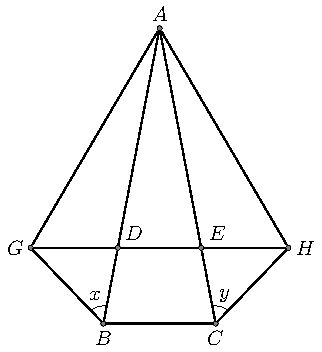
\includegraphics[scale=0.8]{figura}
  \end{minipage}
\end{Problema}

\begin{Solucion}
  
\end{Solucion}

\begin{Problema}{12}
  Se pintan las caras de un cubo, cada una de blanco o negro. �De
  cu�ntas maneras distintas se puede pintar el cubo? (Dos maneras de
  pintar el cubo se consideran iguales si se ven id�nticas girando
  adecuadamente el cubo).
\end{Problema}

\begin{Solucion}
  
\end{Solucion}

\begin{Problema}{13}
  Encuentra el �ltimo d�gito de
  $$
  2012^{(2013^{2014})}- (2012^{2013})^{2014}.
  $$
\end{Problema}

\begin{Solucion}
  
\end{Solucion}

%%% Local Variables: 
%%% mode: latex
%%% TeX-master: "libro"
%%% End: 


\end{document}


% lo que sigue ayuda cuando se edita en Emacs

%%% Local Variables: 
%%% mode: latex
%%% TeX-master: t
%%% TeX-PDF-mode: t
%%% TeX-source-correlate-mode: t
%%% eval: (set-input-method "spanish-prefix")
%%% End: 